% Тут используется класс, установленный на сервере Papeeria. На случай, если
% текст понадобится редактировать где-то в другом месте, рядом лежит файл matmex-diploma-custom.cls
% который в момент своего создания был идентичен классу, установленному на сервере.
% Для того, чтобы им воспользоваться, замените matmex-diploma на matmex-diploma-custom
% Если вы работаете исключительно в Papeeria то мы настоятельно рекомендуем пользоваться
% классом matmex-diploma, поскольку он будет автоматически обновляться по мере внесения корректив
%

% По умолчанию используется шрифт 14 размера. Если нужен 12-й шрифт, уберите опцию [14pt]
\documentclass[14pt]{matmex-diploma}
%\documentclass[14pt]{matmex-diploma-custom}


\usepackage{listings}
\usepackage{color}
 
\definecolor{dkgreen}{rgb}{0,0.6,0}
\definecolor{gray}{rgb}{0.5,0.5,0.5}
\definecolor{mauve}{rgb}{0.58,0,0.82}
\definecolor{gray}{rgb}{0.4,0.4,0.4}
\definecolor{darkblue}{rgb}{0.0,0.0,0.6}
\definecolor{lightblue}{rgb}{0.0,0.0,0.9}
\definecolor{cyan}{rgb}{0.0,0.6,0.6}
\definecolor{darkred}{rgb}{0.6,0.0,0.0}


\lstset{
  basicstyle=\ttfamily\footnotesize,
  columns=fullflexible,
  showstringspaces=false,
  numbers=left,                   % where to put the line-numbers
  numberstyle=\tiny\color{gray},  % the style that is used for the line-numbers
  stepnumber=1,
  numbersep=5pt,                  % how far the line-numbers are from the code
  backgroundcolor=\color{white},      % choose the background color. You must add \usepackage{color}
  showspaces=false,               % show spaces adding particular underscores
  showstringspaces=false,         % underline spaces within strings
  showtabs=false,                 % show tabs within strings adding particular underscores
  frame=none,                   % adds a frame around the code
  rulecolor=\color{black},        % if not set, the frame-color may be changed on line-breaks within not-black text (e.g. commens (green here))
  tabsize=2,                      % sets default tabsize to 2 spaces
  captionpos=b,                   % sets the caption-position to bottom
  breaklines=true,                % sets automatic line breaking
  breakatwhitespace=false,        % sets if automatic breaks should only happen at whitespace
  title=\lstname,                   % show the filename of files included with \lstinputlisting;
                                  % also try caption instead of title  
  commentstyle=\color{gray}\upshape
}


\lstdefinelanguage{XML}
{
  morestring=[s][\color{mauve}]{"}{"},
  morestring=[s][\color{black}]{>}{<},
  morecomment=[s]{<?}{?>},
  morecomment=[s][\color{dkgreen}]{<!--}{-->},
  stringstyle=\color{black},
  identifierstyle=\color{lightblue},
  keywordstyle=\color{red},
  morekeywords={workbook, workbookPr, sheets, sheet, worksheet, cols, col, sheetData, row, c, v, mergeCells, mergeCell, pageMargins, pageSetup, tableParts, tablePart}% list your attributes here
}
\renewcommand{\lstlistingname}{Листинг}

\begin{document}
% Год, город, название университета и факультета предопределены,
% но можно и поменять.
% Если англоязычная титульная страница не нужна, то ее можно просто удалить.
\filltitle{ru}{
    chair              = {кафедра системного программирования},
    title              = {Реализация библиотеки для потоковой обработки .xlsx файлов},
    % Здесь указывается тип работы. Возможные значения:
    %   coursework - Курсовая работа
    %   diploma - Диплом специалиста
    %   master - Диплом магистра
    %   bachelor - Диплом бакалавра
    type               = {coursework},
    position           = {студента},
    group              = 344,
    author             = {Свитков Сергей Андреевич},
    supervisorPosition = {ст. преп\, к.т.н.},
    supervisor         = {Литвинов Ю.\,В.},
}
\maketitle
\tableofcontents
% У введения нет номера главы
\section*{Введение}
В современном мире большой популярностью пользуются многопользовательские веб-приложения. Приложения такого рода могут использоваться для самых разнообразных целей --- от совместного редактирования документов несколькими пользователями до анализа различной статистики операторами связи.

Одну из категорий веб-приложений представляют проекты в сфере телекоммуникаций и биллинга. Такие приложения используются операторами связи для анализа различной статистики по действиям абонентов: перемещения между зонами роуминга, количество входящих/исходящих вызовов, и т.д.

Для формирования отчётов требуется формат представления данных, предоставляющий строгое структурирование. К таким можно отнести JSON, XML, XLSX. Однако, следует принять во внимание, что отчетность или статистика, представленная в таком формате, может использоваться как при взаимодействии различных компонент приложения или различных приложений, так и для анализа человеком. Преимущество формата XLSX в том, что для открытия таких файлов существуют общеизвестные решения (Microsoft Excel, OpenOffice Calc, Google Sheets). 

Таким образом, возникает необходимость в библиотеке, которая позволила бы формировать документы формата XLSX. Следует отметить, что, поскольку объем данных не ограничен, а веб-приложения являются многопользовательскими, то необходимо формировать файл в потоковом режиме, то есть, держать в оперативной памяти только ограниченное количество данных. 

Исходя из сформулированных требований было принято решение проанализировать существующие решения в данной области и, в случае отстутствия подходящей реализации, создать свою библиотеку для решения подобных задач.
\section{Обзор существующих решений}
Задача формирования документов формата XLSX не является новой, имеется ряд существующих библиотек.
\subsection{Apache POI}
    Библиотека Apache POI (далее --- просто POI)предоставляет средства как для формирования, так и для чтения файлов формата .xlsx . До версии 3.8 в библиотеке отсутствовала поддержка потоковой обработки файлов. Несмотря на то, что, начиная с версии 3.8, появилась поддержка потоковой обработки, некоторые проблемы с использованием оперативной памяти остались. Так, некоторые операции над документами всё равно можно проводить только храня целый документ в памяти. К недостаткам библиотеки можно отнести отсутствие возможности задать условия автоматического создания новых страниц в документе, а так же отсутствие полной документации и примеров использования.
    
    Было проведено тестирование библиотеки на количество памяти, требуемое для формирования XLSX файла размером в 1 млн рядов из 50 колонок. Результаты на [рис. 1] //построить график. Из эксперимента можно сделать выводы о том, что, несмотря на наличие возможности потокового формирования файла, с памятью всё равно есть проблемы. 
    
    На момент начала данной работы не было известно о том, что в POI реализована поддержка потоковой обработки документов, что во многом и послужило мотивацией для данной задачи. После анализа последней версии библиотеки было решено реализовать собственный алгоритм потокового формирования документов и сравнить полученную реализацию с POI по производительности.
    
\subsection{SJXLSX}
    Библиотека SJXLSX --- разработка коммьюнити. Документации в проекте крайне мало, к тому же последнее обновление в репозитории было сделано в 2015м году. Был проведен эксперимент по проверке на количество затрачиваемой памяти, результаты эксперимента [рис. 2] // ещё один график. Из эксперимента можно сделать выводы о том, что по количеству используемой операционной памяти при генерации файла данная реализация является крайне неэффективной.
    
\subsection{Итоги обзора}
    Исходя из результатов обзора было принято решение о реализации библиотеки для потоковой генерации файлов и последующем сравнении её с двумя существующими решениями.
    
\section{Постановка задачи}
Целью данной работы является разработка библиотеки для потоковой обработки файлов формата xlsx и сравнение её с существующими реализациями.
Для достижения этой цели были поставлены следующие задачи:
\begin{itemize}
    \item сформулировать подход, который будет использоваться для реализации библиотеки;
    \item реализовать библиотеку;
    \item провести апробацию полученной реализации;
    \item сравнить полученную реализацию с существующими по метрикам:
    \begin{itemize}
        \item потребление RAM при создании документа;
        \item скорость работы;
    \end{itemize}
    \item разместить исходный код и примеры использования библиотеки на github;
\end{itemize}

\section{Анализ формата XLSX}
Перед началом реализации библиотеки было необходимо изучить структуру формата XLSX
Формат XLSX был создан в декабре 2006 года при участии Microsoft, Ecma, ISO/IEC. К сожалению, документации по стандарту MS-XLSX крайне мало, в открытом доступе можно найти только два стандарта: ISO/IEC 29500 (2008) и ECMA-376 1st edition (2006). Эти документы имеют крайне большой объем (порядка 7 тысяч страниц), и на их изучение ушло бы большое количество времени. Для формата XLSX так же существует другой стандарт, Open Office XML. В отличие от стандарта MS-XLSX, данный стандарт довольно хорошо документирован, поэтому было принято решение формировать документы в соответствии с данным стандартом.

Формат XLSX представляет собой ZIP-архив с XML файлами. Его структура (рис. \ref{xlsx_tree}) представляет собой следующий набор файлов и директорий:
\begin{itemize}
    \item \texttt{Content\_Types}.xml --- типы контента в архиве и пути к ним;
    \item \texttt{\_rels} --- зависимости между файлами внутри архива;
    \item docProps --- метаданные: имя автора, дата создания, ...;
    \item xl --- директория с основными файлами архива: workbook, страницы, стили, таблицы;
\end{itemize}

\begin{figure*}
     \centering
     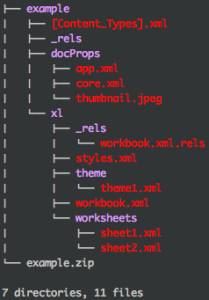
\includegraphics{xlsx_tree.png}
     \caption{Структура формата XLSX}\label{xlsx_tree}
\end{figure*}

Рассмотрим более подробно основные компоненты архива: Workbook и Worksheet.
\subsection{Workbook}
Workbook представляет собой XML-файл, который не содержит данных файла, но содержит следующие мета-данные: ссылки на отдельные Worksheet и их свойства. Пример файла workbook.xml: листинг \ref{list1}. Контент документа содержится непосредственно в Worksheets.
\subsection{Worksheet}
Worksheet содержат данные, из которых и состоит документ. Worksheet может иметь один из следующих форматов: grid, chart, dialog sheet. Наиболее популярным и хорошо задокументированным является grid, рассмотрим его более подробно. 

Grid представляет собой "сетку" из "клеток" (cells) с данными. Каждая клетка может содержать какой-то определенный тип данных: числа, булевские переменные, формулы, и т.д.. Для оптимизации использования памяти строковые значения хранятся не в теле самой клетки, а в отдельной части документа. Это позволяет минимизировать дупликацию строк. Пример файла worksheet.xml (листинг \ref{list2})

Закончив анализ формата XLSX можно приступить к реализации библиотеки.
\section{Реализация}
В данной секции будут описаны алгоритм работы и архитектура библиотеки. Библиотека была реализована на языке Java с использованием системы сборки Maven. Исходный код реализации библиотеки опубликован на Github https://github.com/protei-rnd/oxml-doc. Работа велась под учётной записью likeanowl. Код реализации опубликован под лицензией MIT.
\subsection{Алгоритм}
Было принято решение реализовать следующий алгоритм для генерации файлов формата XLSX:
\begin{itemize}
    \item для каждой страницы создавать временный файл;
    \item хранить в RAM только один ряд (во время создания);
    \item после создания добавлять ряд во временный файл страницы;
    \item после завершения формирования документа --- записывать данные из временных файлов в основной файл;
    \item для экономии дискового пространства сжимать временные файлы.
\end{itemize}

\subsection{Архитектура}
Для реализации предлагаемого алгоритма была реализована следующая архитектура (рис. \ref{arch.png}).
//картинка с диаграммой
Основными элементами приложения являются классы WorkbookWriter и Worksheet. StreamConsumer служит для хранения списка временных файлов, генерируемых при создании документа, а так же позволяет создать InputStream из хранимых файлов. Класс ConnInfo служит для связи SmartOutputStream и StreamConsumer. SmartOutputStream служит для создания OutputStream из временных файлов и записи в них. SheetDescriptor используется связи Worksheet и StreamConsumer. 

Таким образом, полный цикл формирования документа выглядит следующим образом: 
\begin{itemize}
    \item WorkbookWriter создаёт новую страницу, создавая для неё SheetDescriptor, StreamConsumer и SmartOutputStream. Из OutputStream, полученного из SmartOutputStream, создаётся ZipOutputStream для нового временного файла. Созданная страница помечается как готовая к записи.
    \item После создания страницы к ней можно добавлять ряды. Каждый ряд обрабатывается, применяются стили, если они были заданы для ряда, пишется заголовок файла, если он ещё не был записан. В том случае, когда задано ограничение на максимальное количество рядов для одной страницы, происходит автоматическое разбиение и в WorkbookWriter создается новый экземпляр Workheet.
    \item После завершения формирования документа, происходит формирование архива с XML файлами. Это делается путём обхода SheetDescriptor, созданных для страниц документа. Из временных файлов при помощи StreamConsumer создается SequenceInputStream, контент из данного потока пишется в соответствующий странице файл архива. 
\end{itemize}
В репозитории с исходным кодом были размещены примеры использования библиотеки.
\section{Апробация}
Было принято решение сравнить полученную реализацию библиотеки с существующими решениями по следующим метрикам: количество потребляемой при генерации файла оперативной памяти и скорость работы.
Эксперименты проводились на машине с конфигурацией: 
\begin{itemize}
    \item CPU --- Intel i7-7700
    \item RAM --- DDR4 2400 MHz, 16 Gb
    \item SSD --- SATA 3, 340 MB/s
\end{itemize}
//построить график

% У заключения нет номера главы
\section*{Заключение}
В ходе данной работы были достигнуты следующие результаты:
\begin{itemize}
    \item реализована библиотека для потоковой записи файлов формата XLSX;
    \item проведена апробация реализации;
    \item проведено сравнение реализации с существующими по метрикам:
    \begin{itemize}
        \item потребление RAM при создании документа;
        \item скорость работы;
    \end{itemize}
    \item исходный код и примеры использования библиотеки опубликованы на github;
    \item сборка библиотеки опубликована в maven-central (ещё нет).
\end{itemize}
\section*{Листинги}
\begin{lstlisting}[language=XML, caption={Пример файла workbook.xml},captionpos=b, label=list1]
<workbook . . .>
    . . .
    <workbookPr . . ./>
    <sheets>
        <sheet name="sheet1" r:id="rId1">
        <sheet name="sheet2" r:id="rId2">
        <sheet name="sheet3" r:id="rId3">
    </sheets>
    . . .
</workbook>
\end{lstlisting}

\begin{lstlisting}[language=XML, caption={Пример файла worksheet.xml},captionpos=b, label=list2]
<worksheet . . .>
. . .
    <cols>
        <col min="1" max="1" width="26.140625" customWidth="1"/>
            . . .
        </cols>
        
        <sheetData>
            <row r="1">
            <c r="A1" s="1" t="s">
            <v>0</v>
            . . .
            </c>
            </row>
            . . .
        </sheetData>
        . . .
        
        <mergeCells count="1">
        <mergeCell ref="B12:J16"/>
        </mergeCells>
        
        <pageMargins . . ./>
        <pageSetup . . ./>
        
        <tableParts ccount="1">
        <tableParts count="1">
    </tablePart r:id="rId2"/>
</worksheet>
\end{lstlisting}

\setmonofont[Mapping=tex-text]{CMU Typewriter Text}
\bibliographystyle{ugost2008ls}
\bibliography{diploma.bib}
\end{document}
